\section{Background}
% Delete the text and write your Theory/ Background Information here:
%------------------------------------

\subsection{Reinforcement Learning}

Reinforcement learning is defined as the problem that an agent tries to solve by learning behaviour through trial and error with its environment. In other words programming an agent through rewards and punishments rather than how to specifically solve the task itself\cite{kaelbling1996reinforcement} as depicted in figure \ref{figRL}.
\begin{figure}[H]
    \centering
    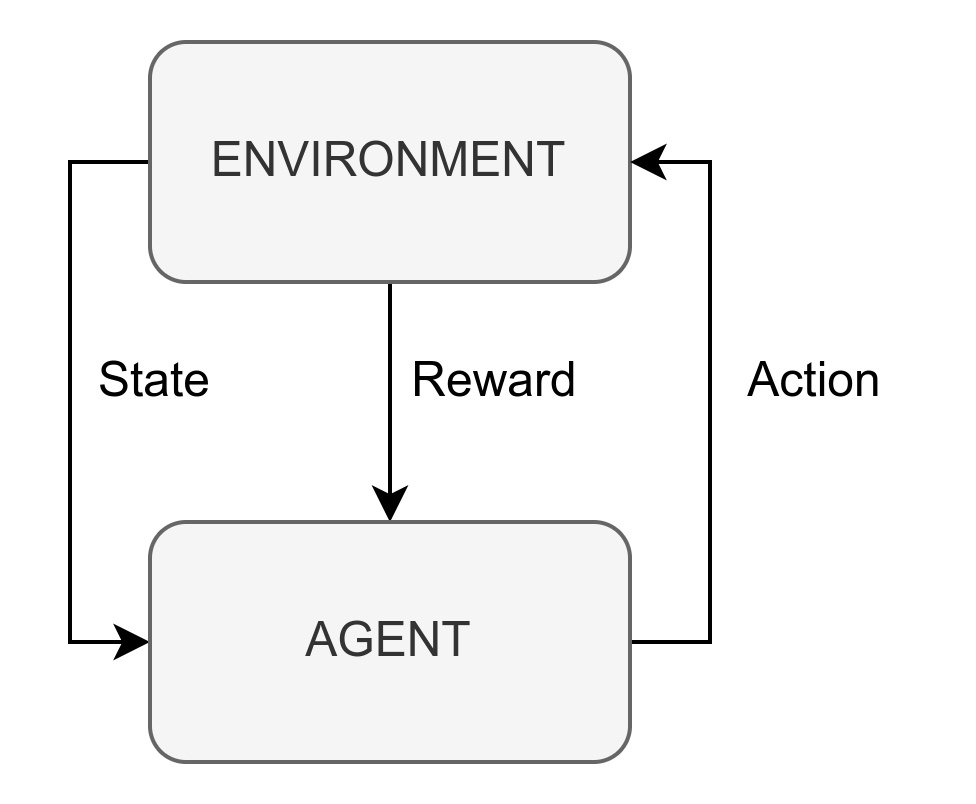
\includegraphics [scale = 0.2]{Images/RL_graph.png}
    \caption{Graph representing reinforcement learning}
    \label{figRL}
\end{figure}
%It can be devided into two strategies for solving said problems. The first strategy involves searching the space or state-action pairs for in order to find which work better in the environment. The second technique is estimating the utillity of a particular action. 
The first concept crucial for reinforcement learning is the \textit{reward function} which is objective feedback from the environment. It is usually scalar values that are associate with state action pairs. High rewards are usually associate by state-action pairs which beneficial for the agent to be situated in whereas negative rewards would then be disadvantageous states or \textit{hazardous} for the agent to be in. Essentially what is good and bad for the agent in the environment. The sole objective of the agent is then to maximize this reward\cite{sutton1999reinforcement}.

Naturally we have to define \textit{state} and \textit{action}, which compared to the rest of the concepts have a very general definition. That being the latter is a descision of some sort and the former a factor that has to be taken into consideration when taking an action. 

\subsubsection{Temporal difference learning}

A central class of methods reinforcement learning is \textit{temporal difference learning}. It refers to a class of methods which the learning is based on the difference between temporally successive predictions. It aims to adjust the learner's current expectation for the present input pattern so that it more accuratly aligns with the subsequent prediction at the following time step. Unlike Monte carlo methods and other methods in temporal learning updates its estimated value function at every step. \cite{tesauro1995temporal}. 

In temporal learning there are several subcmethods or rather algorithms such as SARSA ,Q learning, TD-Lambda and more \cite{eiben2007reinforcement}.\\

\subsubsection{Q learning}
Q learning is an algorithm where the environment can be constituted by a controlled Markov process where the agent is controlling it \cite{watkins1992q}. The agent chooses an action and accordingly gets rewarded for it. Q-learning uses the Markov chains to calculate the max reward that can be accumulated by the next state action and updates towards that as shown in the equation below.

\begin{equation} \label{eqQ}
    { Q(s,a) := Q(s,a) + \eta [r + \gamma \max Q(s',a') - Q(s,a)]}
\end{equation}

Equation \ref{eqQ} is the \textit{value} or \textit{update} equation which is responsible for mapping the different states based on their estimated long term reward in Q learning. Here $Q(s,a)$ is the current state of the agent $r$ is the reward, $\eta$ is the learning rate and $Q(s',a')$ is the next state. An important variable here is $\gamma$ which represent the discount factor. This is used to limit the Markov chain to a limited finite number so they don't end up infinite. This controls how many steps into the future the agent will try ot estimate. 


\subsection{Genetic Algorithms}

Genetic algorithms are computational models based on the concept of evolution as seen in biology. Similarly to how organisms evolve by natural selection and sexual reproduction, programs can also simulate these processes and behave in a similar fashion to organisms in order to solve a specific problem. In a general sense natural selection is the process which determins which individuals get to survive by some test of fitness. After the best fitted are selected the creation or reproduction of the next generation starts. Reproduction is then the method in which the mixing of genes in the remaining population happens and gets passed to the offspring \cite{holland1992genetic}.
\begin{figure}[H]
    \centering
    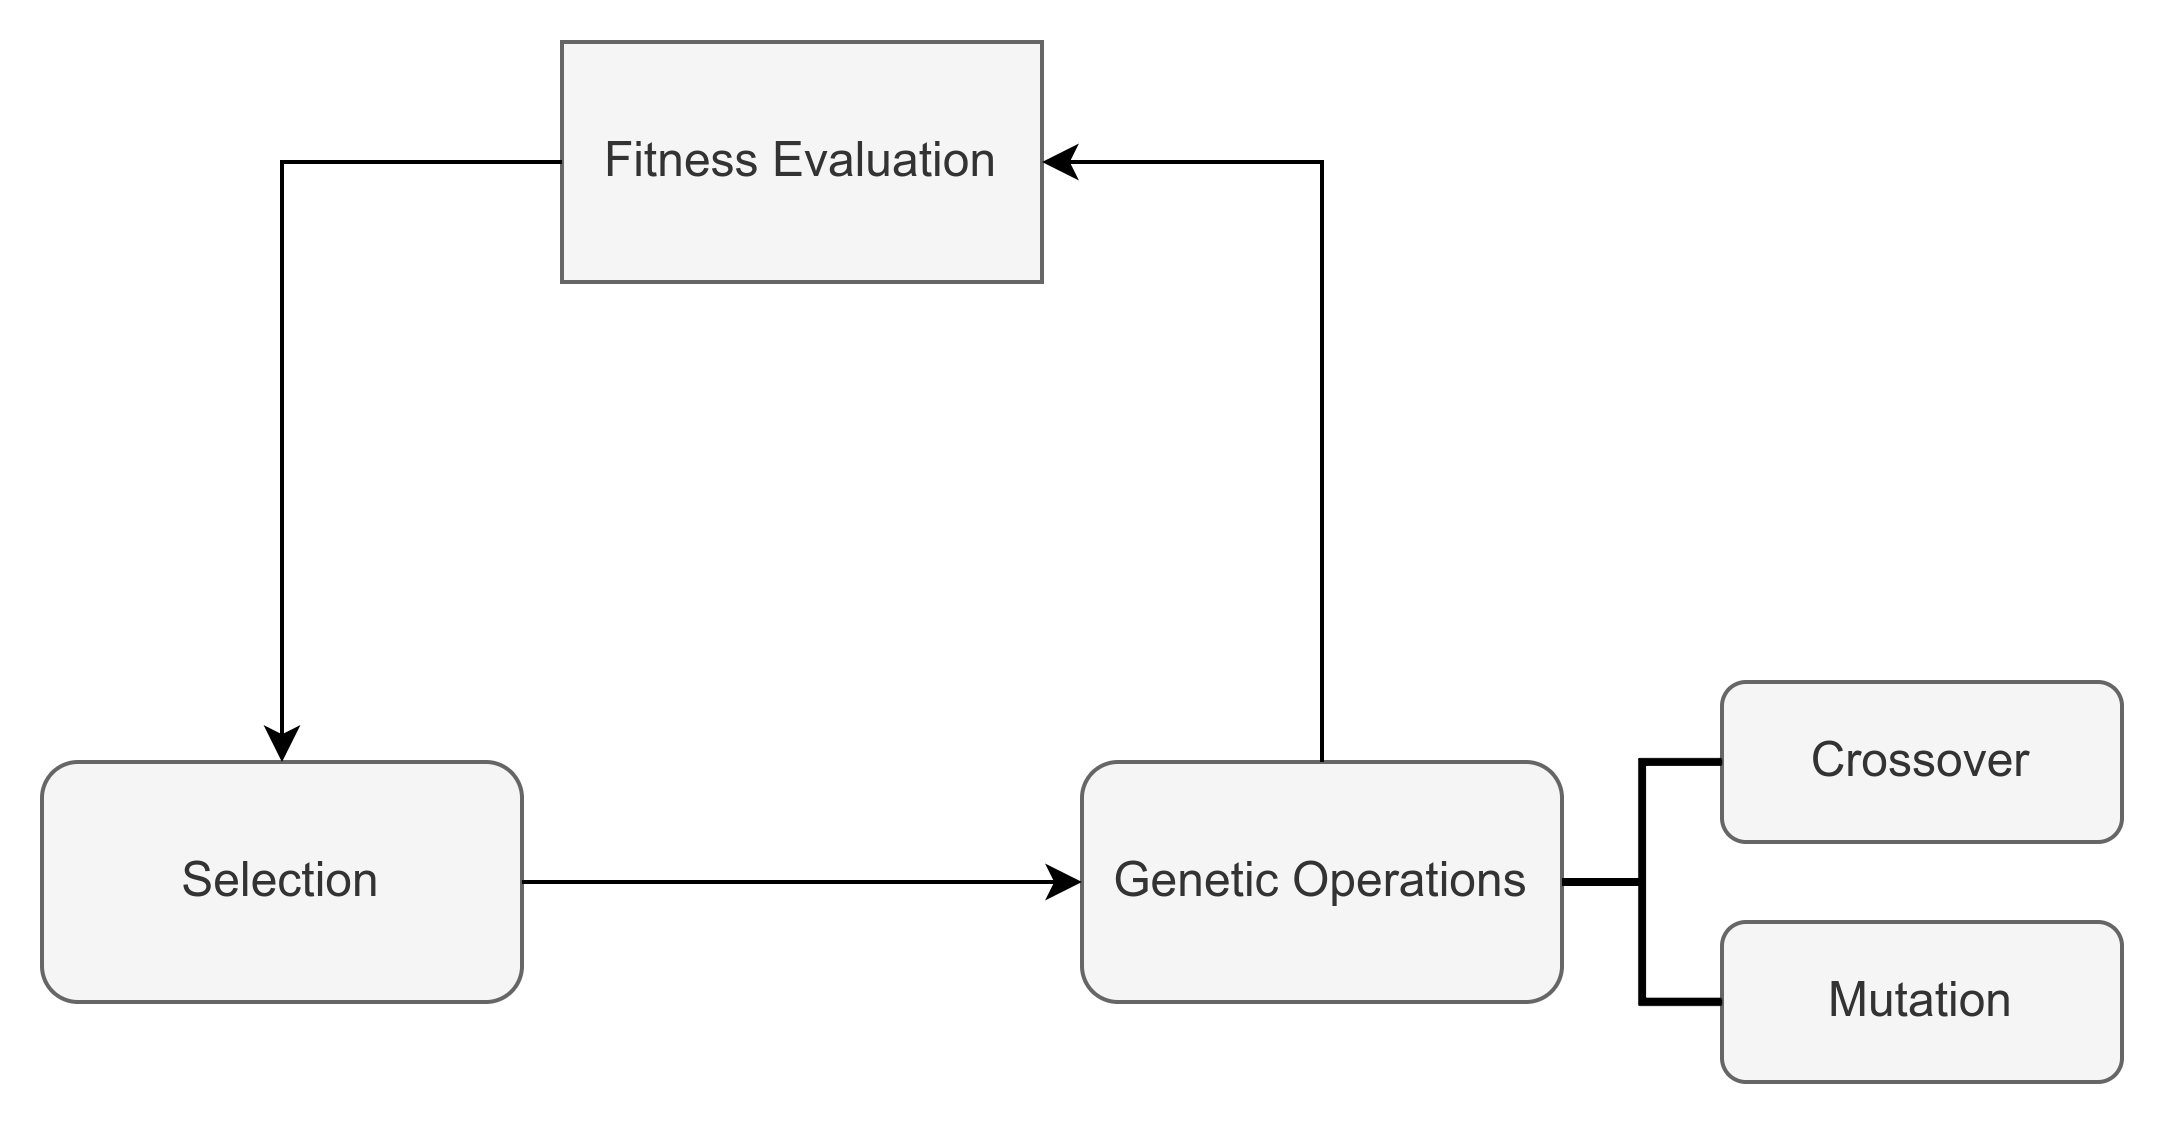
\includegraphics [scale = 0.08]{Images/GA_graph.png}
    \caption{visual representation of genetic algorithms}
    \label{figGA}
\end{figure}

By starting with a population of individuals wich are creaated randomly we have an initial population with variation amongst the individuals. The DNA wich is essentialy the code of the gene can be represented by a string of bits. These string bits can thought as potential solutions to the problem. Due to the variation in the population some individuals vill be better \textit{fit} which then will be selected to remain. In the final stage the remaining individuals will mix their bit strings to produce individuals for the next generation. These steps will be continually done fore some number of generations \cite{forrest1996genetic}. 

It is important however that we reduce the genetic drift and keep track of hte best solutions that have been produced by the previous generation. To do that we employ a method called Elitism. In ellitism compared with traditional reproductiion the most fitting individual are copied to the next generation without any alteration. In that way the best solution of each generation is alway preserved and adds selective preassure and improve convergence speed \cite{du2018elitism}.
